 \documentclass[xcolor=dvipsnames, aspectratio=169, 10pt]{beamer}
% \usepackage{vntex}
\usetheme[sectionpage=progressbar,subsectionpage=progressbar]{metropolis}
\usepackage{tikz}
\usetikzlibrary{arrows, decorations.pathreplacing}
\usetikzlibrary{backgrounds}
\usepackage{caption}
\usepackage{animate}
\usepackage{bm}
% \setbeamertemplate{caption}[numbered]
% \usepackage{subcaption}

\usepackage[lined,commentsnumbered]{algorithm2e}
\usepackage{etoolbox}
\beamertemplatenavigationsymbolsempty
% \useinnertheme{circles}
%\useoutertheme{split}

\definecolor{gustave}{HTML}{1d2392}

\definecolor{background}{HTML}{274150}
\definecolor{sbackground}{HTML}{1d2392}
\definecolor{main-text}{HTML}{80A07C}
\definecolor{enumercolor}{HTML}{A4CCE0}
\definecolor{progress-bar}{HTML}{E6CBA0}\usecolortheme[named=sbackground]{structure} % define for item color, commented Jan 4,2024

%% TITLE PAGE 
\title[]{BRANCH AND BOUND ALGORITHM \\ FOR VERTEX COVER PROBLEM}
\subtitle{Optimization Project}

\AtBeginDocument{
	\author[Minh]{
		\begin{tabular}{lll}
			\textit{\small Students:} & \small CHAU Dang Minh \\
			& \small LAM Nhat Quan \\
            \vspace{.5cm}\\
		\end{tabular}
	}
}
% \institute[Limoges]{
% 	{
% 		Gustave Eiffel University \\
% 	}
% }
% TOC
\setbeamertemplate{section in toc}[circle]
\setbeamercolor{section in toc}{bg=sbackground!40, fg=black} % change color section item
 \setbeamerfont{section number projected}{size=\large}
% ENUM
  % \setbeamercolor{item projected}{bg=red!70!black,fg=white}
  \setbeamercolor{frametitle}{fg=sbackground,bg=sbackground!40} % change color bar
  \setbeamercolor{background canvas}{bg=white} % change color frame
  \setbeamercolor{normal text}{fg=black} % change text color
\setbeamercolor{progress bar}{fg=progress-bar!110,bg=progress-bar!50} % change progress bar color
    \setbeamertemplate{enumerate items}[circle]
    \setbeamerfont{itemize item projected}{size=\huge}
        \setbeamerfont{item projected}{size=\large}
% CAPTION
\setbeamertemplate{caption}{\raggedright\insertcaption\par}
% LOGO
\usepackage{textpos} 

\addtobeamertemplate{frametitle}{}{%
	\begin{textblock*}{100mm}(\textwidth,-.9cm)
		% \includegraphics[height=.7cm,width=.7cm]{logo.png}
\end{textblock*}}
\usepackage{eso-pic}
\usepackage{pgf}
\titlegraphic{
	\begin{picture}(0,0)
		\put(420,5){\makebox(0,0)[rt]{\includegraphics[width=5cm]{logo.png}}}
	\end{picture}
}
\setbeamertemplate{bibliography item}{\insertbiblabel}
\newcommand{\nologo}{\setbeamertemplate{logo}{}}
% HEADLINE
%\setbeamertemplate{headline}{}
% FOOTLINE
\setbeamercolor{custom1}{fg=black,bg=mycolor}
\setbeamercolor{custom2}{fg=black, }
\setbeamercolor{custom3}{fg=black,}
\setbeamerfont{footline}{series=\bfseries}%, family=\ttfamily}
\setbeamertemplate{footline}{%
	\leavevmode%
% 	\begin{beamercolorbox}[wd=0.25\textwidth, sep=0.4em, center]{custom1}%
% 		\strut \quad\insertshortauthor \quad (\insertshortinstitute)
% 	\end{beamercolorbox}%
% 	\begin{beamercolorbox}[wd=0.45\textwidth, sep=0.4em, center]{custom2}%
% 		\strut \insertshorttitle
% 	\end{beamercolorbox}%
	\begin{beamercolorbox}[wd=1\textwidth, sep=0.4em, right]{custom3}%
		\strut \insertframenumber/\inserttotalframenumber
	\end{beamercolorbox}%
}
% Thank you slide
\makeatletter
\let\beamer@writeslidentry@miniframeson=\beamer@writeslidentry%
\def\beamer@writeslidentry@miniframesoff{%
	\expandafter\beamer@ifempty\expandafter{\beamer@framestartpage}{}% does not happen normally
	{%else
		% removed \addtocontents commands
		\clearpage\beamer@notesactions%
	}
}
\newcommand*{\miniframeson}{\let\beamer@writeslidentry=\beamer@writeslidentry@miniframeson}
\newcommand*{\miniframesoff}{\let\beamer@writeslidentry=\beamer@writeslidentry@miniframesoff}
\makeatother

\input{commands.tex}

\usepackage[most]{tcolorbox}
\tcbuselibrary{breakable,skins}

% Shared counter for all theorem-like environments
\newcounter{mytheoremcounter}

\newtcolorbox{mydefinition}[1][]{%
  enhanced,
  title={Definition \stepcounter{mytheoremcounter}\themytheoremcounter\ifstrempty{#1}{}{ (#1)}},
  % attach boxed title to top left={yshifttext=-1mm},
  colback=white,
  colframe=gustave!50!black,
  fonttitle=\bfseries,
  boxed title style={
    size=small,
    colback=gustave!50!black,
    colframe=gustave!50!black,
  },
}

\newtcolorbox{mytheorem}[1][]{%
  enhanced,
  title={Theorem \stepcounter{mytheoremcounter}\themytheoremcounter\ifstrempty{#1}{}{ (#1)}},
  % attach boxed title to top left={yshifttext=-1mm},
  colback=white,
  colframe=gustave!50!black,
  fonttitle=\bfseries,
  boxed title style={
    size=small,
    colback=gustave!50!black,
    colframe=gustave!50!black,
  },
}

\newtcolorbox{myproposition}[1][]{%
  enhanced,
  title={Proposition \stepcounter{mytheoremcounter}\themytheoremcounter\ifstrempty{#1}{}{ (#1)}},
  % attach boxed title to top left={yshifttext=-1mm},
  colback=white,
  colframe=gustave!50!black,
  fonttitle=\bfseries,
  boxed title style={
    size=small,
    colback=gustave!50!black,
    colframe=gustave!50!black,
  },
}


% DOCUMENT
\begin{document}
\date{}
\begin{frame}[noframenumbering,plain]
  \titlepage
\end{frame}

\begin{frame}{Outline}
  \tableofcontents
\end{frame}

\section{Problem}

\begin{frame}{Original Vertex Cover}
    Given a graph $G = (V,E)$, a \textbf{vertex cover} is a subset of vertices $S \subseteq V$ such that for every edge $\{u,v\} \in E$, at least one of $u$ or $v$ is in $S$.

    The \textbf{minimum vertex cover} problem seeks to find a vertex cover of the smallest possible size.

    Let $w: V \to \mathbb{R}^+$ be a weight function assigning a positive weight to each vertex. The \textbf{weighted minimum vertex cover} problem aims to find a vertex cover $S$ that minimizes the total weight
    $$w(S):=\sum_{v \in S} w(v).$$

    % The \textbf{Minimum Vertex Cover} \textbf{(MVC)} is an extensively studied problem with numerous applications in operation research. MVC is a well-known NP-Complete problem.

    % The problem seeks the smallest set of vertices such that every edge in the graph has at least one endpoint in it, and hence forming the MVC solution.

\end{frame}

\begin{frame}{Integer Programming Formulation}
    The weighted minimum vertex cover problem can be formulated as the following integer programming problem:
    \begin{equation}
        \begin{array}{ll@{}ll}
            \text{minimize}   & \displaystyle\sum\limits_{v\in V} w(v) & x_{v}               &                      \\
            \text{subject to} & \displaystyle                          & x_{u} + x_v \geq 1, & \forall \{u,v\}\in E \\
                              &                                        & x_{v} \in \{0,1\}.  &
        \end{array}
        \tag{IP}
    \end{equation}

    The vertex cover corresponding to a solution $x$ is given by $S = \{ v \in V : x_v = 1 \}$.

    But solving (IP) is NP-hard in general.
\end{frame}

\begin{frame}{Linear Programing Relaxation}
    Algorithms make use of the LP-relaxation
    \begin{equation}
        \begin{array}{ll@{}ll}
            \text{minimize}   & \displaystyle\sum\limits_{v\in V} w(v) & x_{v}                             &                      \\
            \text{subject to} & \displaystyle                          & x_{u} + x_v \geq 1,               & \forall \{u,v\}\in E \\
                              &                                        & \textcolor{gustave}{x_{v} \ge 0.} &                      \\
        \end{array}
        \tag{LP}
    \end{equation}

    \textbf{Note:} Every optimal solution always has $x_v\le 1$, since if $x_v>1$ for some vertex $v$, we can set $x_v=1$ without violating any constraints and get a better solution.
\end{frame}

% \begin{frame}{Introduction}
%     \begin{mytheorem}[Nemhauser-Trotter]
%         There exists an optimal solution \textit{OPT} with the following properties:
%         \begin{enumerate}[(a)]
%             \item \textit{OPT} is a subset of $(V_1 \cup V_{1/2})$,
%             \item \textit{OPT} includes all of $V_1$.
%         \end{enumerate}
%     \end{mytheorem}

%     The Nemhauser–Trotter theorem guarantees that optimal LP extreme points satisfy $x_v \in \{ 0,1,1/2 \}$.
% \end{frame}

% \begin{frame}{Introduction}
%     In this project, we try to make use of the Branch-and-Bound (BnB) algorithm to solve the MVC, using \textbf{'pulp'} library to implement the algorithm, and then we use \textbf{'networkx'} library to check the result with the maximum-matching, since we already have:
%     \begin{align*}
%         \textrm{maximum\_matching}(G) \leq \textrm{minimum\_VC}(G).
%     \end{align*}

%     Moreover, we also try to improve the result with the strong BnB algorithm.
% \end{frame}
\section{Solution Properties}

\begin{frame}{Optimal Solutions to (LP)}
  \begin{mytheorem}[Nemhauser-Trotter]
    Let $x$ be an extreme point of the polytope defined by the constrains of (LP) we have $x_v \in \{0, \frac{1}{2}, 1\}$ for every $v \in V$.
  \end{mytheorem}
\end{frame}

\begin{frame}[allowframebreaks]{Optimal Solutions to (LP)}
  \textit{Proof.} Let $x$ be an extreme point. Let $U\subset V$ be the set of vertices such that $x_v \notin \{0, \frac{1}{2}, 1\}$ for every $v \in U$. Suppose for contradiction that $U$ is non-empty.

  \begin{center}
    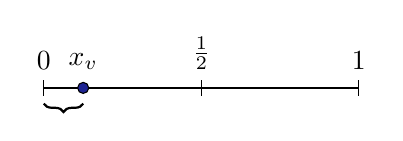
\begin{tikzpicture}
      % Draw the main line segment
      \draw[thick, -] (0,0) -- (4,0);

      % Mark the key points
      \draw[] (0,0) node[above=3pt] {$0$};
      \draw[] (2,0) node[above=3pt] {$\frac{1}{2}$};
      \draw[] (4,0) node[above=3pt] {$1$};

      % Add a variable point x_v
      \draw[fill=gustave] (0.5,0) circle (2pt) node[above=3pt] {$x_v$};

      % Add tick marks
      \draw (0,0.1) -- (0,-0.1);
      \draw (2,0.1) -- (2,-0.1);
      \draw (4,0.1) -- (4,-0.1);

      % Add curly brace from 0 to x_v
      \draw[thick,decorate,decoration={brace,amplitude=3pt,mirror}] (0,-0.2) -- (0.5,-0.2);
    \end{tikzpicture}
    \hspace{1cm}
    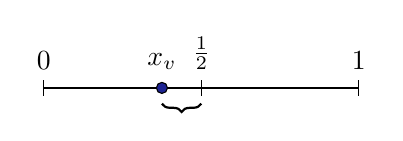
\begin{tikzpicture}
      % Draw the main line segment
      \draw[thick, -] (0,0) -- (4,0);

      % Mark the key points
      \draw[] (0,0) node[above=3pt] {$0$};
      \draw[] (2,0) node[above=3pt] {$\frac{1}{2}$};
      \draw[] (4,0) node[above=3pt] {$1$};

      % Add a variable point x_v
      \draw[fill=gustave] (1.5,0) circle (2pt) node[above=3pt] {$x_v$};

      % Add tick marks
      \draw (0,0.1) -- (0,-0.1);
      \draw (2,0.1) -- (2,-0.1);
      \draw (4,0.1) -- (4,-0.1);

      % Add curly brace from 0 to x_v
      \draw[thick,decorate,decoration={brace,amplitude=3pt,mirror}] (1.5,-0.2) -- (2,-0.2);
    \end{tikzpicture}

    \vspace{0.5cm}

    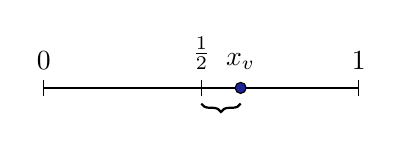
\begin{tikzpicture}
      % Draw the main line segment
      \draw[thick, -] (0,0) -- (4,0);

      % Mark the key points
      \draw[] (0,0) node[above=3pt] {$0$};
      \draw[] (2,0) node[above=3pt] {$\frac{1}{2}$};
      \draw[] (4,0) node[above=3pt] {$1$};

      % Add a variable point x_v
      \draw[fill=gustave] (2.5,0) circle (2pt) node[above=3pt] {$x_v$};

      % Add tick marks
      \draw (0,0.1) -- (0,-0.1);
      \draw (2,0.1) -- (2,-0.1);
      \draw (4,0.1) -- (4,-0.1);

      % Add curly brace from 0 to x_v
      \draw[thick,decorate,decoration={brace,amplitude=3pt,mirror}] (2,-0.2) -- (2.5,-0.2);
    \end{tikzpicture}
    \hspace{1cm}
    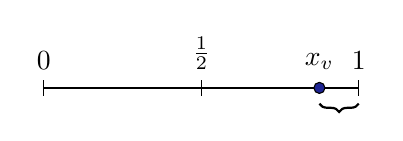
\begin{tikzpicture}
      % Draw the main line segment
      \draw[thick, -] (0,0) -- (4,0);

      % Mark the key points
      \draw[] (0,0) node[above=3pt] {$0$};
      \draw[] (2,0) node[above=3pt] {$\frac{1}{2}$};
      \draw[] (4,0) node[above=3pt] {$1$};

      % Add a variable point x_v
      \draw[fill=gustave] (3.5,0) circle (2pt) node[above=3pt] {$x_v$};

      % Add tick marks
      \draw (0,0.1) -- (0,-0.1);
      \draw (2,0.1) -- (2,-0.1);
      \draw (4,0.1) -- (4,-0.1);

      % Add curly brace from 0 to x_v
      \draw[thick,decorate,decoration={brace,amplitude=3pt,mirror}] (3.5,-0.2) -- (4,-0.2);
    \end{tikzpicture}
  \end{center}

  Take the minimum distance $\epsilon$ from $x_v$ to the closest of $\{0, \frac{1}{2}, 1\}$ for every $v \in U$ i.e.
  $$\epsilon = \min_{v \in U} \min \left\{ |x_v - 0|, \left| x_v - \frac{1}{2} \right|, |x_v - 1| \right\}.$$

  Perturb $x$ at each $v \in U$ by $ \epsilon$ by two different ways to get two new solutions $x^+$ and $x^-$ defined as follows:
  $$x^+(v) = \begin{cases}
      x_v + \epsilon & \text{if } v \in U \text{ and } x_v < \frac{1}{2}, \\
      x_v - \epsilon & \text{if } v \in U \text{ and } x_v > \frac{1}{2}, \\
      x_v            & \text{otherwise}
    \end{cases} \quad \quad
    x^-(v) = \begin{cases}
      x_v - \epsilon & \text{if } v \in U \text{ and } x_v < \frac{1}{2}, \\
      x_v + \epsilon & \text{if } v \in U \text{ and } x_v > \frac{1}{2}, \\
      x_v            & \text{otherwise}.
    \end{cases}$$
  We have $x=\dfrac{1}{2}(x^+ + x^-)$.

  \break

  Two see that both $x^+$ and $x^-$ are feasible, there are two cases

  \begin{itemize}
    \item[(i)] If an edge $uv \in E$ has $x_u < \frac{1}{2}$ and $x_v > \frac{1}{2}$, then
          $$x^+_u + x^+_v = x^-_u + x^-_v = x_u + x_v \ge 1.$$

          \begin{center}
            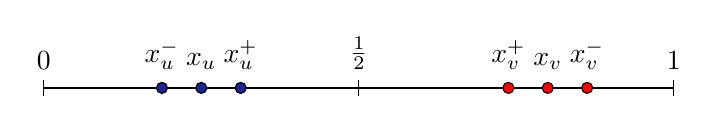
\begin{tikzpicture}
              % Draw the main line segment
              \draw[thick, -] (0,0) -- (8,0);

              % Mark the key points
              \draw[] (0,0) node[above=3pt] {$0$};
              \draw[] (4,0) node[above=3pt] {$\frac{1}{2}$};
              \draw[] (8,0) node[above=3pt] {$1$};

              % Add tick marks
              \draw (0,0.1) -- (0,-0.1);
              \draw (4,0.1) -- (4,-0.1);
              \draw (8,0.1) -- (8,-0.1);

              % Original points x_u and x_v
              \draw[fill=gustave] (2,0) circle (2pt) node[above=3pt] {$x_u$};
              \draw[fill=red] (6.4,0) circle (2pt) node[above=3pt] {$x_v$};

              % x^+ points (red)
              \draw[fill=gustave] (2.5,0) circle (2pt) node[above=3pt] {$x^+_u$};
              \draw[fill=red] (5.9,0) circle (2pt) node[above=3pt] {$x^+_v$};

              % x^- points (blue)
              \draw[fill=gustave] (1.5,0) circle (2pt) node[above=3pt] {$x^-_u$};
              \draw[fill=red] (6.9,0) circle (2pt) node[above=3pt] {$x^-_v$};
            \end{tikzpicture}
          \end{center}

          The constraint $x_u + x_v \ge 1$ is satisfied for both $x^+$ and $x^-$ since the sum remains at least 1.
    \item[(ii)] If an edge $uv \in E$ has both $x_u, x_v > \frac{1}{2}$. Then $x^+_u, x^-_u, x^+_v, x^-_v \ge \frac{1}{2}$. Hence

          $$x^+_u + x^+_v \ge 1 \text{ and } x^-_u + x^-_v \ge 1.$$

          \begin{center}
            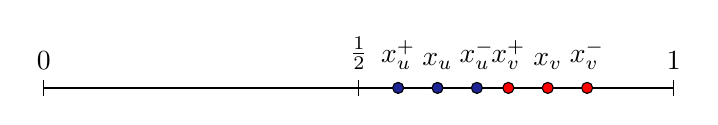
\begin{tikzpicture}
              % Draw the main line segment
              \draw[thick, -] (0,0) -- (8,0);

              % Mark the key points
              \draw[] (0,0) node[above=3pt] {$0$};
              \draw[] (4,0) node[above=3pt] {$\frac{1}{2}$};
              \draw[] (8,0) node[above=3pt] {$1$};

              % Add tick marks
              \draw (0,0.1) -- (0,-0.1);
              \draw (4,0.1) -- (4,-0.1);
              \draw (8,0.1) -- (8,-0.1);

              % Original points x_u and x_v
              \draw[fill=gustave] (5,0) circle (2pt) node[above=3pt] {$x_u$};
              \draw[fill=red] (6.4,0) circle (2pt) node[above=3pt] {$x_v$};

              % x^+ points (red)
              \draw[fill=gustave] (4.5,0) circle (2pt) node[above=3pt] {$x^+_u$};
              \draw[fill=red] (5.9,0) circle (2pt) node[above=3pt] {$x^+_v$};

              % x^- points (blue)
              \draw[fill=gustave] (5.5,0) circle (2pt) node[above=3pt] {$x^-_u$};
              \draw[fill=red] (6.9,0) circle (2pt) node[above=3pt] {$x^-_v$};
            \end{tikzpicture}
          \end{center}


  \end{itemize}

  \break

  Since there is an optimal solution to (LP) that is also an extreme point, we conclude there exists an optimal solution $x^*$ such that $x^*_v \in \{0, \frac{1}{2}, 1\}$ for every $v \in V$.

  Define the set $S_1$ of vertices with value 1 in $x^*$ and similarly the sets $S_0$ and $S_{1/2}$.

  \begin{center}
    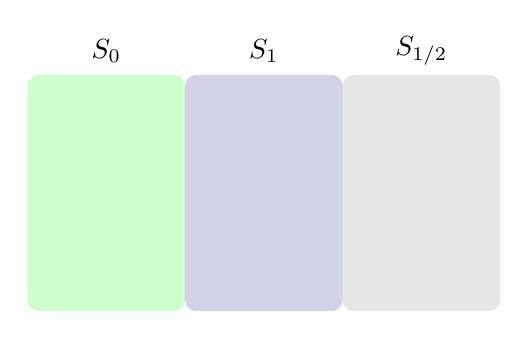
\begin{tikzpicture}
      % Box for S_1
      \node at (1,3.3) {$S_0$};
      \fill[green, opacity=0.2, rounded corners] (0,0) rectangle (2,3);

      % Box for S_0
      \node at (3,3.3) {$S_1$};
      \fill[gustave, opacity=0.2, rounded corners] (2,0) rectangle (4,3);
      % Box for S_{1/2}
      \node at (5,3.3) {$S_{1/2}$};
      \fill[gray, opacity=0.2, rounded corners] (4,0) rectangle (6,3);

      \segment{0.75}{0.25}{2.75}{0.25}
      \segment{3}{0.75}{3}{2.75}
      \segment{3.25}{0.25}{5.25}{0.25}
      \segment{5}{0.75}{5}{2.75}
    \end{tikzpicture}
  \end{center}
  Possible cases of edges in $E$ are shown above.
\end{frame}

\begin{frame}{Solutions to (IP) from (LP)}
  \begin{mytheorem}[Nemhauser-Trotter]
    Let $x^*$ be an optimal solution to (LP).  Then there exists an optimal solution of (IP) that generates a vertex cover $S\subset V$ such that $S_1 \subset S \subset S_1 \cup S_{1/2}$.
  \end{mytheorem}
\end{frame}

\begin{frame}{Vertex Cover from (LP)}
  \textit{Proof.} Firstly, we show that $S\subset S_1 \cup S_{1/2}$. Suppose not i.e. $C_0 = S\cap S_0$ is not empty.

  For every vertex $v \in C_0$, there can only be edges between $v$ and vertices in $S_1$.
  \begin{center}
    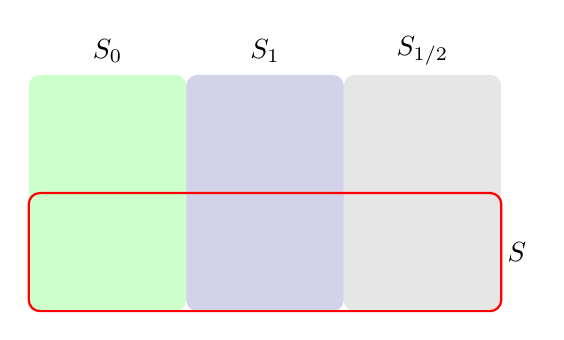
\begin{tikzpicture}
      % Box for S_1
      \node at (1,3.3) {$S_0$};
      \fill[green, opacity=0.2, rounded corners] (0,0) rectangle (2,3);

      % Box for S_0
      \node at (3,3.3) {$S_1$};
      \fill[gustave, opacity=0.2, rounded corners] (2,0) rectangle (4,3);
      % Box for S_{1/2}
      \node at (5,3.3) {$S_{1/2}$};
      \fill[gray, opacity=0.2, rounded corners] (4,0) rectangle (6,3);

      % Box for S (vertex cover) - covers bottom half
      \draw[thick, red, rounded corners] (0,0) rectangle (6,1.5);
      \node at (6.2,0.75) {$S$};
    \end{tikzpicture}
  \end{center}
\end{frame}

\begin{frame}[allowframebreaks]{Vertex Cover from (LP)}
  Edges from $C_0$ to $\overline{C}_1=S_1\setminus S$ are covered once by $S$.
  \begin{center}
    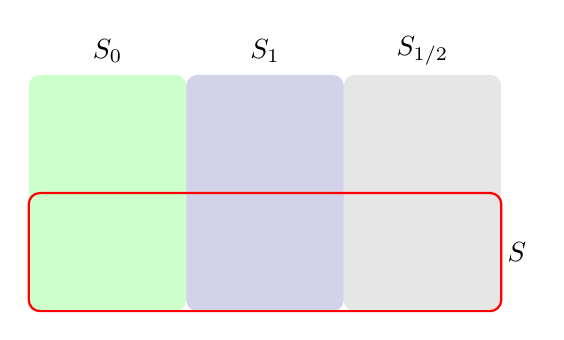
\begin{tikzpicture}
      % Box for S_1
      \node at (1,3.3) {$S_0$};
      \fill[green, opacity=0.2, rounded corners] (0,0) rectangle (2,3);

      % Box for S_0
      \node at (3,3.3) {$S_1$};
      \fill[gustave, opacity=0.2, rounded corners] (2,0) rectangle (4,3);
      % Box for S_{1/2}
      \node at (5,3.3) {$S_{1/2}$};
      \fill[gray, opacity=0.2, rounded corners] (4,0) rectangle (6,3);

      % Box for S (vertex cover) - covers bottom half
      \draw[thick, red, rounded corners] (0,0) rectangle (6,1.5);
      \node at (6.2,0.75) {$S$};

      % Edge from C_0 to \overline{C}_1
      \segment{1}{0.75}{3}{2.25}
    \end{tikzpicture}
  \end{center}
  \break
  If $w(\overline{C}_1) \le w(C_0)$, we can get a better solution by choosing $\overline{C}_1$ instead of $C_0$.
  \begin{center}
    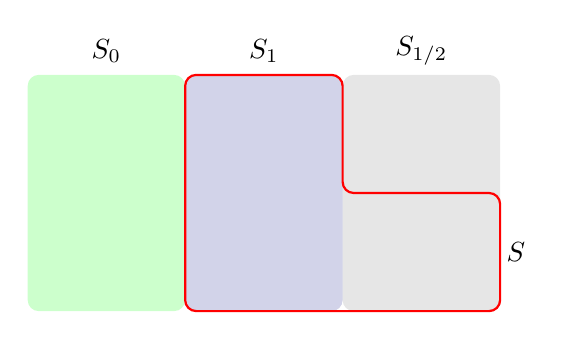
\begin{tikzpicture}
      % Box for S_1
      \node at (1,3.3) {$S_0$};
      \fill[green, opacity=0.2, rounded corners] (0,0) rectangle (2,3);

      % Box for S_0
      \node at (3,3.3) {$S_1$};
      \fill[gustave, opacity=0.2, rounded corners] (2,0) rectangle (4,3);
      % Box for S_{1/2}
      \node at (5,3.3) {$S_{1/2}$};
      \fill[gray, opacity=0.2, rounded corners] (4,0) rectangle (6,3);

      % Box for S (vertex cover) - covers S_1 and bottom half of S_{1/2}
      \draw[thick, red, rounded corners] (2,0) -- (2,3) -- (4,3) -- (4,1.5) -- (6,1.5) -- (6,0) -- cycle;
      \node at (6.2,0.75) {$S$};

      % Edge from C_0 to \overline{C}_1
      \segment{1}{0.75}{3}{2.25}
    \end{tikzpicture}
  \end{center}

  If $w(C_0) < w(\overline{C}_1)$, we use the perturbation technique again: add a small $\epsilon$ to every vertex in $C_0$ and subtract $\epsilon$ from every vertex in $\overline{C}_1$ to get a better feasible solution to (LP), contradicting the optimality of $x^*$.

  \break

  Now we prove that $S_1 \subset S$. Suppose not, i.e. $\overline{C}_1$ is nonempty. Let $v \in \overline{C}_1$.

  \begin{center}
    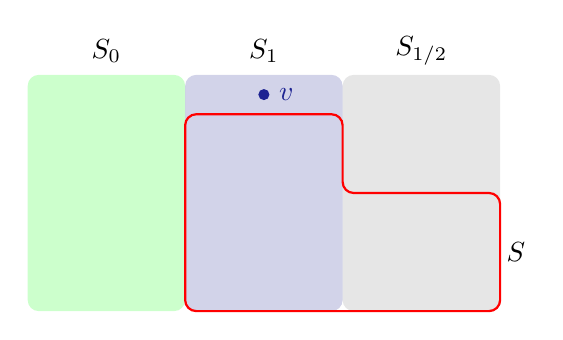
\begin{tikzpicture}
      % Box for S_1
      \node at (1,3.3) {$S_0$};
      \fill[green, opacity=0.2, rounded corners] (0,0) rectangle (2,3);

      % Box for S_0
      \node at (3,3.3) {$S_1$};
      \fill[gustave, opacity=0.2, rounded corners] (2,0) rectangle (4,3);
      % Box for S_{1/2}
      \node at (5,3.3) {$S_{1/2}$};
      \fill[gray, opacity=0.2, rounded corners] (4,0) rectangle (6,3);

      % Box for S (vertex cover) - covers S_1 and bottom half of S_{1/2}
      \draw[thick, red, rounded corners] (2,0) -- (2,2.5) -- (4,2.5) -- (4,1.5) -- (6,1.5) -- (6,0) -- cycle;
      \node at (6.2,0.75) {$S$};

      \fill[gustave] (3,2.75) circle (2pt) node[right=2pt] {$v$};
    \end{tikzpicture}
  \end{center}

  If $w(v) = 0$, include $v$ in $S$ anyway (the value of (IP) does not change).

  Consider the case $w(v) > 0$. Note that $v$ cannot have neighbors in $S_0$. Hence, we can decrease $x_v$ from 1 to $\frac{1}{2}$ and get a better feasible solution to (LP), contradicting the optimality of $x^*$.
\end{frame}




\section{Branch and Bound for Vertex Cover}
\begin{frame}{General Algorithm}

  \begin{enumerate}
    \item Maintain the current cost and the current best solution.
    \item Extract $S_0, S_1$ and $S_{1/2}$ from an extreme solution of (LP).
    \item If adding $S_1$ exceeds the current best solution, stop (prune this branch).
    \item If $S_{1/2}$ is empty, update the current best solution if necessary and stop.
    \item Choose a vertex $v \in S_{1/2}$.
    \item Return to step 2 two following graphs in some order:
          \begin{itemize}
            \item Graph with $v$ included in the vertex cover (remove $v$ and its incident edges).
            \item Graph with $v$ excluded from the vertex cover (remove $v$'s neighbors and their incident edges, add $v$ to the current cost).
          \end{itemize}
  \end{enumerate}

  Different strategies for steps 5 and 6 lead to different algorithms.
\end{frame}

\begin{frame}{Experiments}
  We consider three strategies
  \begin{itemize}
    \item Choosing the vertex with the highest degree in $S_{1/2}$ and include it first.
    \item Choosing the vertex with the lowest degree in $S_{1/2}$ and exclude it first.
    \item Fully-strong branching \footnote{Bénichou, Michel, et al. "Experiments in mixed-integer linear programming." Mathematical programming 1.1 (1971): 76-94.}: choose the vertex and the order whose resulting two LP relaxations have the highest total value.
  \end{itemize}
\end{frame}

\begin{frame}

\end{frame}


\begin{frame}[noframenumbering,plain]
  \begin{center}
    \Huge\textbf{Thank you for listening !}
  \end{center}
\end{frame}

\input{sections/appendix.tex}
% \printbsibliography
\end{document}